\section{Empirical Evaluation} \label{Sec:evaluation}
To quantitatively assess the efficacy of our test generation approach, we have conducted a case study, in which we address the following research questions:

\begin{description}[noitemsep]
\item [RQ1] How accurate is \tool in mapping DOM-based assertions to the corresponding \javascript code?
\item [RQ2] How effective is \tool in generating unit test assertions that detect faults?
\item [RQ3] Is our approach more effective than DOM-based assertions written manually by the tester in terms of fault finding capability? 
\item [RQ4] How does our approach compare to the existing mutation-based technique for identifying unit test assertions?
\end{description}

\tool and the experimental data are available for download \cite{atrina-dl}.
\subsection{Objects}
Our study includes four open source \javascript web applications that have \selenium test cases.
%Finding applications with executable Selenium test cases for \javascript applications is a big challenge.
\tabref{objectsTable} presents the experimental objects and their properties. Phormer \cite{phormer} is a photo gallery web application. EnterpriseStore \cite{enterpriseStore} is an asset management web application. WolfCMS \cite{wolfcms} is a content management system, and Claroline \cite{claroline} is a collaborative online learning and course management system. 
\begin{table}
        \caption{Characteristics of the experimental objects.} \label{Table:objectsTable}        
{\scriptsize
\centering
%    \begin{center}
       
      %  \subtable[Experimental subjects and the corresponding exploration data]
            {
           \begin{tabular}{l|l|l|>{\centering}m{1cm}|c} \hline
\thead{ID} &\thead{Name} &\thead{LOC (JS)} &\thead{\# Test Cases} &\thead{\# Assertions}  \\  \hline 

\hline

1  & Phormer & 1.5K & 7 & 18    \\ \hline
           
2 & EnterpriseStore & 57K & 19 & 21  \\ \hline

3 & WolfCMS & 1.3K & 12 & 42  \\ \hline

4 & Claroline & 36K & 23 & 35 \\ \hline

5 & StudyRoom & 10.6K & 12 & 23 \\ \hline

6 & AddressBook & 1.1K & 13 & 14 \\ \hline

7 & Brotherhood & 0.8K & 10 & 10 \\ \hline
\end{tabular}
            }

%\end{center}
}
\vspace{-0.2in} 
\end{table}
\subsection{Setup} \label{Sec:setup}
To address our research questions, we provide the URL as well as the available manually written DOM-based test suite of each experimental object to \tool. Unit level test assertions are then automatically generated by the tool.
\headbf{Accuracy (RQ1)} To evaluate the accuracy of \tool, we measure precision and recall. We manually compare the slices generated by \tool with the \javascript code that is relevant to each assertion. Precision and recall are defined as follows:
\begin{description}[noitemsep, nolistsep, font=\normalfont\itshape]
\item [Precision] is the fraction of lines in a slice produced by \tool, that are actually related to the human-written DOM-based assertion: $\frac{TP}{TP+FP}$ 
\item [Recall] is the fraction of the correct set of related lines of code to each assertion, which is actually present in the slice produced by \tool: $\frac{TP}{TP+FN}$ 
\end{description}
where $TP$ (true positives), $FP$ (false positives), and $FN$ (false negatives) respectively represent the number of lines of code that are correctly reported, falsely reported, and missed to report as related to the DOM-based assertion.
\headbf{Effectiveness (RQ2)} To assess the effectiveness of \tool, we measure the fault finding capability of the assertions generated by the tool. Moreover, to understand the effect of each type of assertion produced by \tool in detecting faults, we compare the fault detection rate of using (1) exclusively explicit assertions, (2) explicit assertions and implicit assertions, and (3) explicit assertions and candidate assertions. Since explicit assertions compose the core body of our assertions, we consider implicit and candidate assertions in conjunction with explicit ones.
       
The experimental objects do not come with a rich version history to apply \tool on real regression changes. Therefore we mimic regression faults by automatically injecting mutations to the application, and evaluate the tool's ability in detecting the seeded faults. We randomly inject 50 first-order mutations into the \javascript code of the applications. The mutation operators are chosen from a list of common operators such as changing the value of a variable, modifying a conditional statement, altering unary operations, as well as common mistakes made by developers when developing a given web application \cite{mirshokraie:tse15}, e.g., changing the ID/tag name passed into DOM access functions such as \code{getElementById} or \code{getElementsByTagName}, and modifying the attribute name/value in \code{setAttribute}. The fault is considered detected if an assertion generated by \tool fails when run on the mutated code, and our manual examination confirms that the failed assertion is detecting the seeded fault.
\headbf{Comparison with human-written DOM-based Assertions (RQ3)} To assess the usefulness of \tool, we compare the human written DOM-based assertions with the unit-level test assertions generated by our approach in terms of fault finding capability.
Similar to RQ2, we perform fault injection on both.
The faults injected into our experimental objects in response to RQ3 are the same as the ones that we seed in applications to answer RQ2.
\headbf{Comparison with Mutation-based Assertion Generation (RQ4)} To assess how \tool performs with respect to the current state-of-the-art oracle generation technique, we compare our tool's fault finding capability with the mutation-based assertion generation approach \cite{mirshokraie:icst15, fraser:tse12}. To generate mutation-based assertions for the \javascript code, we use human-written DOM-based test suite as a means to execute the application and infer the execution traces required for the purpose of mutation analysis. We perform the following steps to generate test assertions using mutation analysis.
\begin{enumerate}[noitemsep, nolistsep]
\item Remove assertions from the human-written DOM-based test suite.
\item Execute the test suite on the original version of the application to obtain execution traces.
\item Inject mutations for the purpose of oracle generation.
\item Execute the human-written test suite on the generated mutants, and produce test oracles by comparing execution traces obtained from the mutants and the original version of the application.
\end{enumerate}
The number of mutants, that are generated to produce test assertions is 50 for each application. Note that the implementation and evaluation of the mutation analysis technique both use mutation operators suggested by \cite{mirshokraie:tse15}. Therefore, our evaluation is biased in favour of mutation-based assertion generation approach over our technique.
\subsection{Results} \label{Sec:results}
\headbf{Effectiveness (RQ1)} \figref{assertionTypeFaultDetec} depicts the fault detection rate achieved by \tool, explicit assertions when used individually and when it is used in conjunction with either implicit assertions or candidate assertions. 

\begin{figure}[!t]
  \centering
  \includegraphics[width=1\hsize]{r-scripts/assertionTypeFaultDetec}
  \vspace{-0.18in} 
  \mycaption{Fault detection rate using different types of generated assertions.}
  \vspace{-0.1in} 
  \label{Fig:assertionTypeFaultDetec}
 
\end{figure}

\headbf{Comparison with human-written DOM-based Assertions (RQ2)}

\begin{figure}[!t]
  \centering
  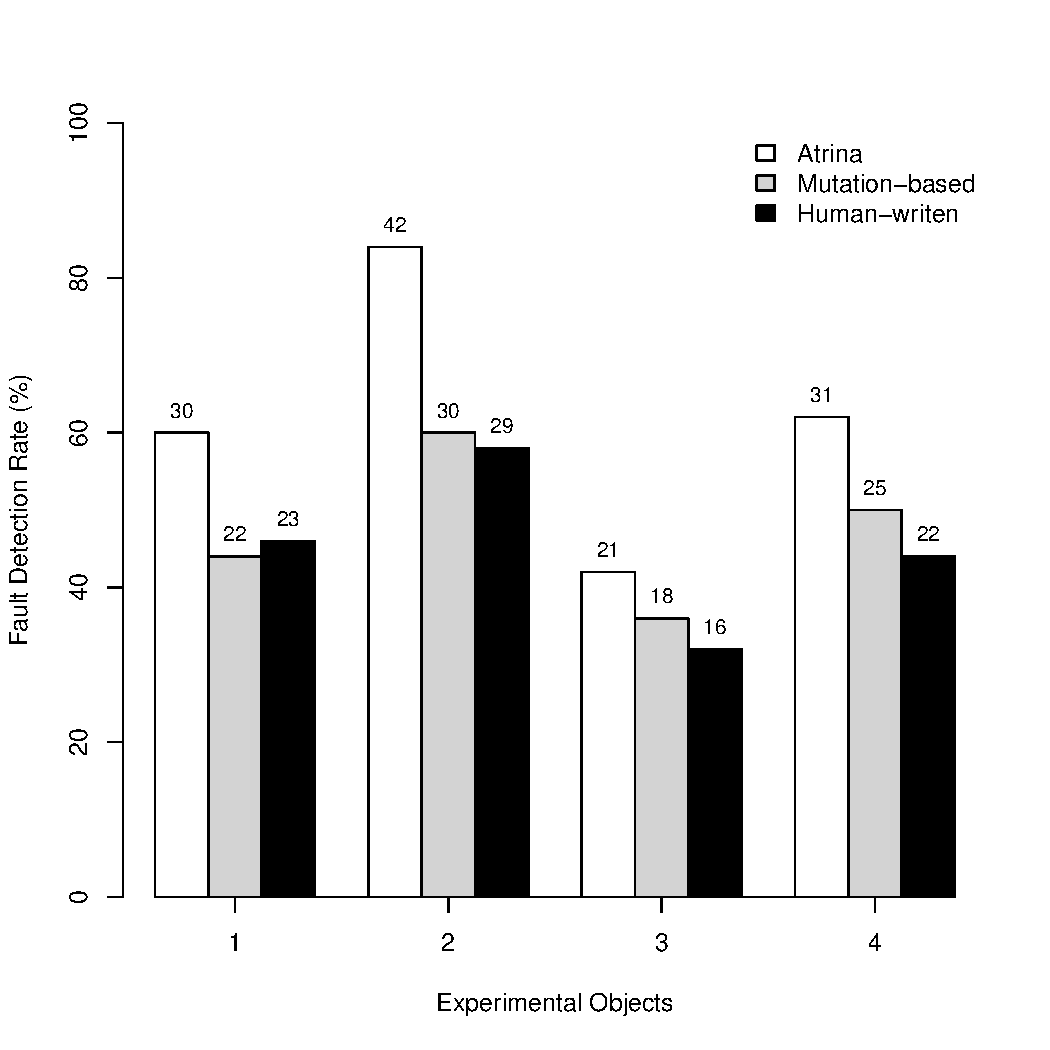
\includegraphics[width=1\hsize]{r-scripts/barplot-faultDetectionRate}
  \vspace{-0.18in}   
  \mycaption{Fault finding capability.}
  \vspace{-0.1in} 
  \label{Fig:faultDetectionRate}

\end{figure}

\headbf{Accuracy (RQ3)}
\begin{table}
        \caption{Accuracy achieved by \tool.} \label{Table:accuracyTable}        
{\scriptsize
\centering
%    \begin{center}
       
      %  \subtable[Experimental subjects and the corresponding exploration data]
            {
           \begin{tabular}{l|l|l|l|l|l} \hline
\theadturn{ID} &\theadturn{\# TP} &\theadturn{\# FP} &\theadturn{\# FN} &\theadturn{Precision (\%)} &\theadturn{Recall (\%)}  \\  \hline 

1  & 174 & 0 & 0 & 100 & 100    \\ \hline
           
2 & 861 & 18 & 162 & 98 & 84  \\ \hline

3 & 193 & 0 & 0 & 100 & 100  \\ \hline

4 & 1446 & 29 & 385 & 98 & 79 \\ \hline

\hline\end{tabular}
            }

%\end{center}
}
%\vspace{-0.2in} 
\end{table}
\headbf{Comparison with Mutation-based Assertion Generation (RQ4)}




\section{Discussion}
\label{Sec:discussion}

% \head{Correlation.} To examine the relationship between the 
% cyclomatic complexity of objects and the number of unique invariants, 
% we used R \cite{?} to calculate the non-parametric
% Spearman correlation coefficients (r) as well as the p-values (p), 
% and plotted the graphs. We present the combinations that
% indicate a possible correlation.\figref{inv-cc} depicts the scatter plot of the
% cyclomatic complexity versus the number of unique invariants. 
% The correlation coefficient ($r = 0.867$, $p = 0.002$) suggests that variables 
% are positively co-related: The higher the cyclomatic complexity, the more unique invariants
% are detected in the application. The reason might be that larger value of cyclomatic complexity 
% implies that more number of decision points are present in the program. Consequently, pushing more 
% restrictions on varibales and parameters of the application may result in inferring more number of
% invariants. 
% \begin{figure}
% \centering
% 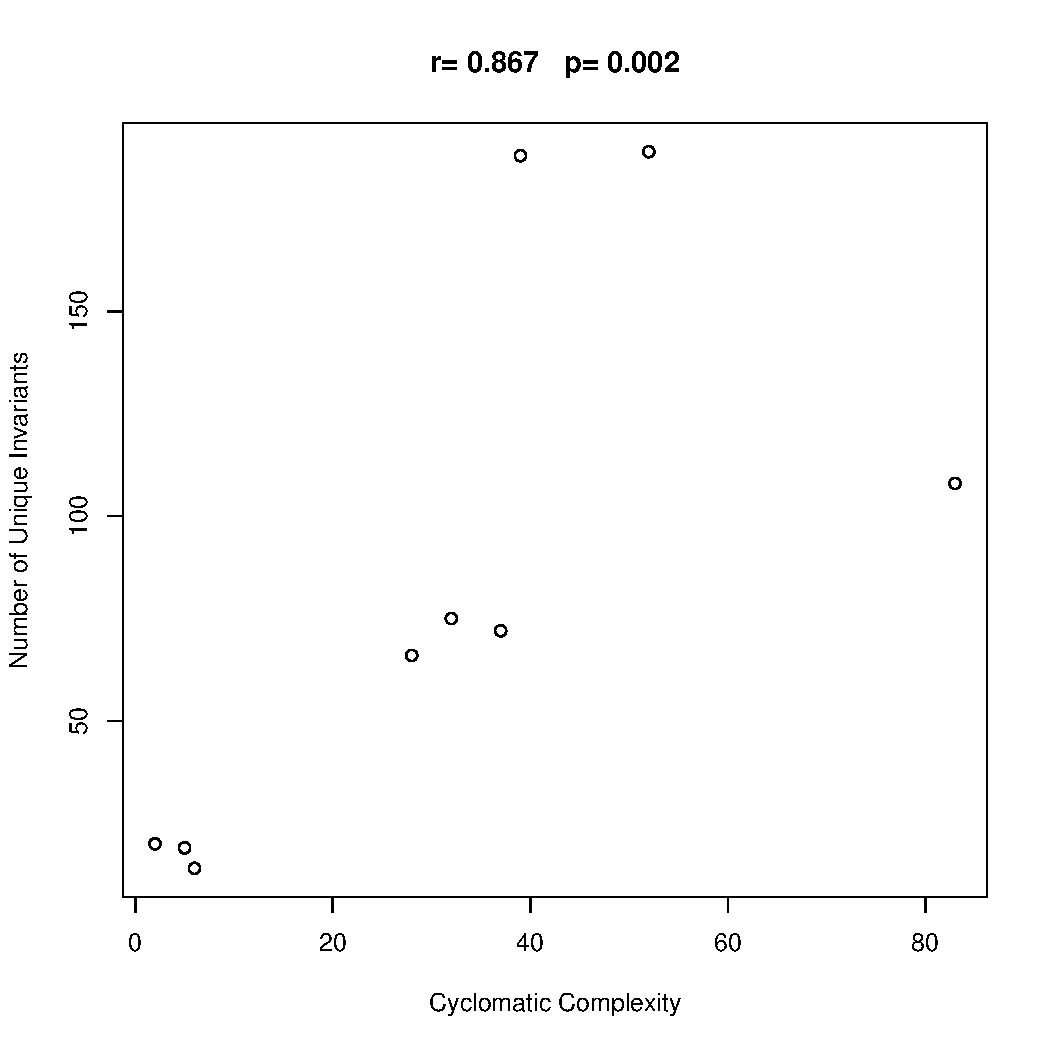
\includegraphics[width=0.7\hsize]{rscripts/inv_cc}
% \mycaption{Scatter plot of the number of unique invariants versus
% cyclomatic complexity. r represents the Spearman correlation coefficient and p is
% the p-value.}
% \label{Fig:inv-cc}
% \vspace{-0.3in}
% \end{figure}
%(1) the precision of comparing two floating point numbers in Daikon;
%The first is concerned with the number of digits in the fractional part of the floating point numbers, which is used by Daikon while comparing two floats. We resolve this by increasing the precision of float comparisons in Daikon configurations.
\head{Unstable Assertions.} As mentioned in \secref{filtering}, we observe a few number of unstable invariant assertions initially, which are removed by our filtering mechanism. By analyzing our trace data, we observe
that such unstable assertions arise mainly because of the 
multiple runtime types of \javascript variables.
This is based on the fact that in \javascript it is possible to change the type of a variable at runtime. However, Daikon treats variables as single type, selects the first observed type, and ignores the subsequent types in the trace data. This results in producing a few number of unstable invariant assertions for \javascript.
We remove such unstable assertions in our filtering step. A drawback of removing these assertions, is that our tool might miss a fault during the regression testing phase.
However, according to our observations, such unstable assertions form only around 5\% of the total generated assertions. Thus, we are still able to achieve high accuracy as presented in the previous section.
    
\head{Limitations.} Our approach is not able to detect syntax errors that are present in the \javascript code. Furthermore, tracing DOM manipulations using APIs other than the standard DOM API or jQuery is currently not supported by \jsart.
Further, a regression fault either directly violates an invariant assertion, or it can violate closely 
related assertions, which have been affected by the fault. However, if the tool is not able to infer any invariants in the  affected scope of the error, it fails to detect the fault. This results in observing a low rate of false negatives as illustrated in \secref{evaluation}. 
     
\head{Revisiting the Assumptions.} As we mentioned in \secref{approach}, we assume that the current version of the web application is bug-free. This is based on the fact that in regression testing a gold standard is always needed as a trusted version for comparing the test results against \cite{Binder:2000} to detect regression faults. However, if the original version of the application does contain an error, the generated assertions might reflect the error as well, and as such they are not able to detect the fault. 
Our second assumption states that the program specifications are unlikely to change frequently in revisions. Here we assume that software programs evolve gradually and regression faults are mostly due to small changes. However, if major upgrades occur in subsequent revisions such that the core specification of the application is affected, the inferred invariants from the original version may not be valid any longer and new invariant assertions need to be generated.

% Competent Programmer Hypothesis (CPH) \cite{acree:mutation1979, demillo:computer1978}. It states that programmers tend to develop programs, which are close to the correct version. Therefore,
% regression faults are mostly due to simple faults occur during small changes in the program. These faults made by competent programmers are merely simple faults such that the applications's behavior is not significanlty affected.


 

\begin{table}[t]
%\vspace{5pt}
        \caption{Manual effort imposed by our approach for deriving stable invariant assertions.}
{\scriptsize
    \begin{center}
       
      %  \subtable[Experimental subjects and the corresponding exploration data]
            {
           \begin{tabular}{c|c|c} \hline
\thead{App ID} & \thead{Total Time (min)} & \thead{Manual Effort (min)} \\  \hline \hline

1  & 13  & 4 \\ \hline %535
           
2  & 11.5 & 3 \\ \hline %502

3 & 15.5  & 5 \\ \hline % 639

4  & 11  & 3 \\ \hline %500

5  & 6.5 & 2.5 \\ \hline %227

6  & 9  & 4.5 \\ \hline %214

7  & 7.5  & 3.5 \\ \hline %244

8  & 6.5  & 2 \\ \hline %278

9  & 18 & 13 \\ \hline %266
\hline\end{tabular}\centering
            }
\label{Table:manualEffort_table}
\end{center}
}  
\vspace{-0.2in} 
\end{table}



\head{Automation Level.} While the testing phase of \jsart is fully automated, the navigation part requires some manual effort. Although the crawling is performed automatically, we do need to manually setup the tool with different crawling configurations per application execution.  Moreover, for each application run, we manually look at the size of the invariant output to decide whether more execution traces (and thus more crawling sessions) are needed.
%Thus, manual effort is concerned with tracing and filtering unstable invaraint assertions, where we need to execute the application 
%per crawling configuration. 
%
We present the manual effort involved with detecting stable invariant assertions in \tabref{manualEffort_table}. 
The table shows the total time, which is the duration time of deriving stable assertions including both automatic and manual parts. 
The reported manual effort contains the amount of time required 
for setting up the tool as well as the manual tasks involved with the navigation part.
The results show the average manual effort is less than 5 minutes.





\subsection{Threats to Validity} \label{Sec:threatsToValidity}
An external threat to the validity of our evaluation is the limited number of \javascript applications used to measure the effectiveness of our approach. We mitigated this threat by using web applications from various domains, code size, and functionality. Another threat concerns validating failed assertions through manual inspection that can be error-prone. To mitigate this threat, we carefully examine the code in which the assertion failed to make sure that the injected fault was responsible for the assertion failure. Moreover, manual computation of the \javascript slices to measure precision and recall is a time intensive task done by the authors of the paper, and thus we acknowledge that it could be error-prone, although we made every effort to mitigate this threat by precisely examining the application's code.

The regression faults we inject to evaluate the effectiveness of \tool may not be realistic. We mitigate this threat by injecting mutations that represent common \javascript applications faults, as well as using real-world web applications, and test cases written by other developers. 

